\documentclass[14pt]{article}
\usepackage[colorlinks,allcolors=blue]{hyperref}
\usepackage{pdfpages}
\usepackage{graphics}
\usepackage{epsfig}
\usepackage{times}
\usepackage{amsmath}
\usepackage{subcaption}
\usepackage{multirow}
\usepackage{gensymb}
\usepackage{array}
\usepackage{float}
\usepackage{indentfirst}
\newcolumntype{P}[1]{>{\centering\arraybackslash}p{#1}}
\usepackage{booktabs, makecell}
\usepackage{diagbox}
\usepackage{float}
\floatstyle{plaintop}
\restylefloat{table}


\topmargin      0.0in
\headheight     0.0in
\headsep        0.0in
\oddsidemargin  0.0in
\evensidemargin 0.0in
\textheight     9.0in
\textwidth      6.5in

\title{{\bf CENG424 Embedded Computer Systems\\Final Exam Project Proposal \\ Spring 2022} \\ Group 9 \\
	\it Project Title: Soil Humidity Meter}


\date{\today}

\begin{document}

\pagestyle{plain}
\pagenumbering{roman}
\maketitle


\begin{figure}[H]
	\centering
	
\includegraphics[ scale = 0.35]{iyte_logo} 
\end{figure}

\textbf{ Group Members}
\begin{itemize}
	\item Student\_1 Arif Burak Demiray \& 250201022
	\item Student\_2 Ramazan Arslan \& 250201023 
	\item Student\_3 Burak Tutumlu \& 250201039
	\item Student\_4 Bekir Yörük \& 250201046
	\item Student\_5 Onur Cihangir \& 250201049
\end{itemize}



\cleardoublepage
\pagenumbering{arabic}

\abstract
In this project, we aim to inform farmers and plant growers about the humidity levels around İzmir and how this moisture level is affected by the factors that contribute to soil fertility, and how this productivity is kept at an optimum level [2]. This project aims to improve over the years and increase humidity data more accurately. In addition, with this project, we will observe how the amount of moisture affects the soils. By analyzing the data in the system where we measure the moisture content of soils in various regions with the tool we built with this project with Arduino, we will be able to observe the moisture-soil productivity relationship and transfer the moisture content to the relevant people.
\cleardoublepage

\section{Introduction}
In this project, we aim to measure the humidity information of the soil with the humidity meter sensor. By transferring this data to a cloud-based system, we aim to determine the difference in humidity between locations and to prepare a data on the factors affecting humidity. In this way, people who are interested in plant and garden works are going to be able to grow their soils in a healthier way, and those who want to access more detailed information about the relationship between soil and humidity are going to be able to develop more accurate products by using our data.

\section{Problem Definition}
One of the biggest problems that people experience while dealing with agriculture and plant breeding is that the factors that contribute to soil fertility cannot be kept at an optimum level. One of the most important of these factors is the humidity level [3]. To measure this humidity level, people used various methods before. To give some examples, Gravimetric method, Electrical Resistance Method etc. But these are methods that are primitive in various aspects such as time or efficiency. With a simple and easy-to-use device, this project intends to give users with information on the soil and the optimal planting period, even without plants [4]. In this scenario, we are going to upload the data we collected with the Arduino and the soil humidity meter to the cloud system and make it accessible from a mobile and online platform. Users are going to be able to see on the mobile app that they have precise humidity information about their plants and when is the optimal time to plant using this solution quickly and simply. They are going to be able to see the humidity levels in the areas where the project is placed on the website. Furthermore, individuals are going to be able to rapidly compare their fields and plants in other areas due to our project, and our project is going to therefore serve as a method of growing plants in line with the circumstances of the site. 



\section{Stages}

\title{\textbf{Sequence Diagram}} 

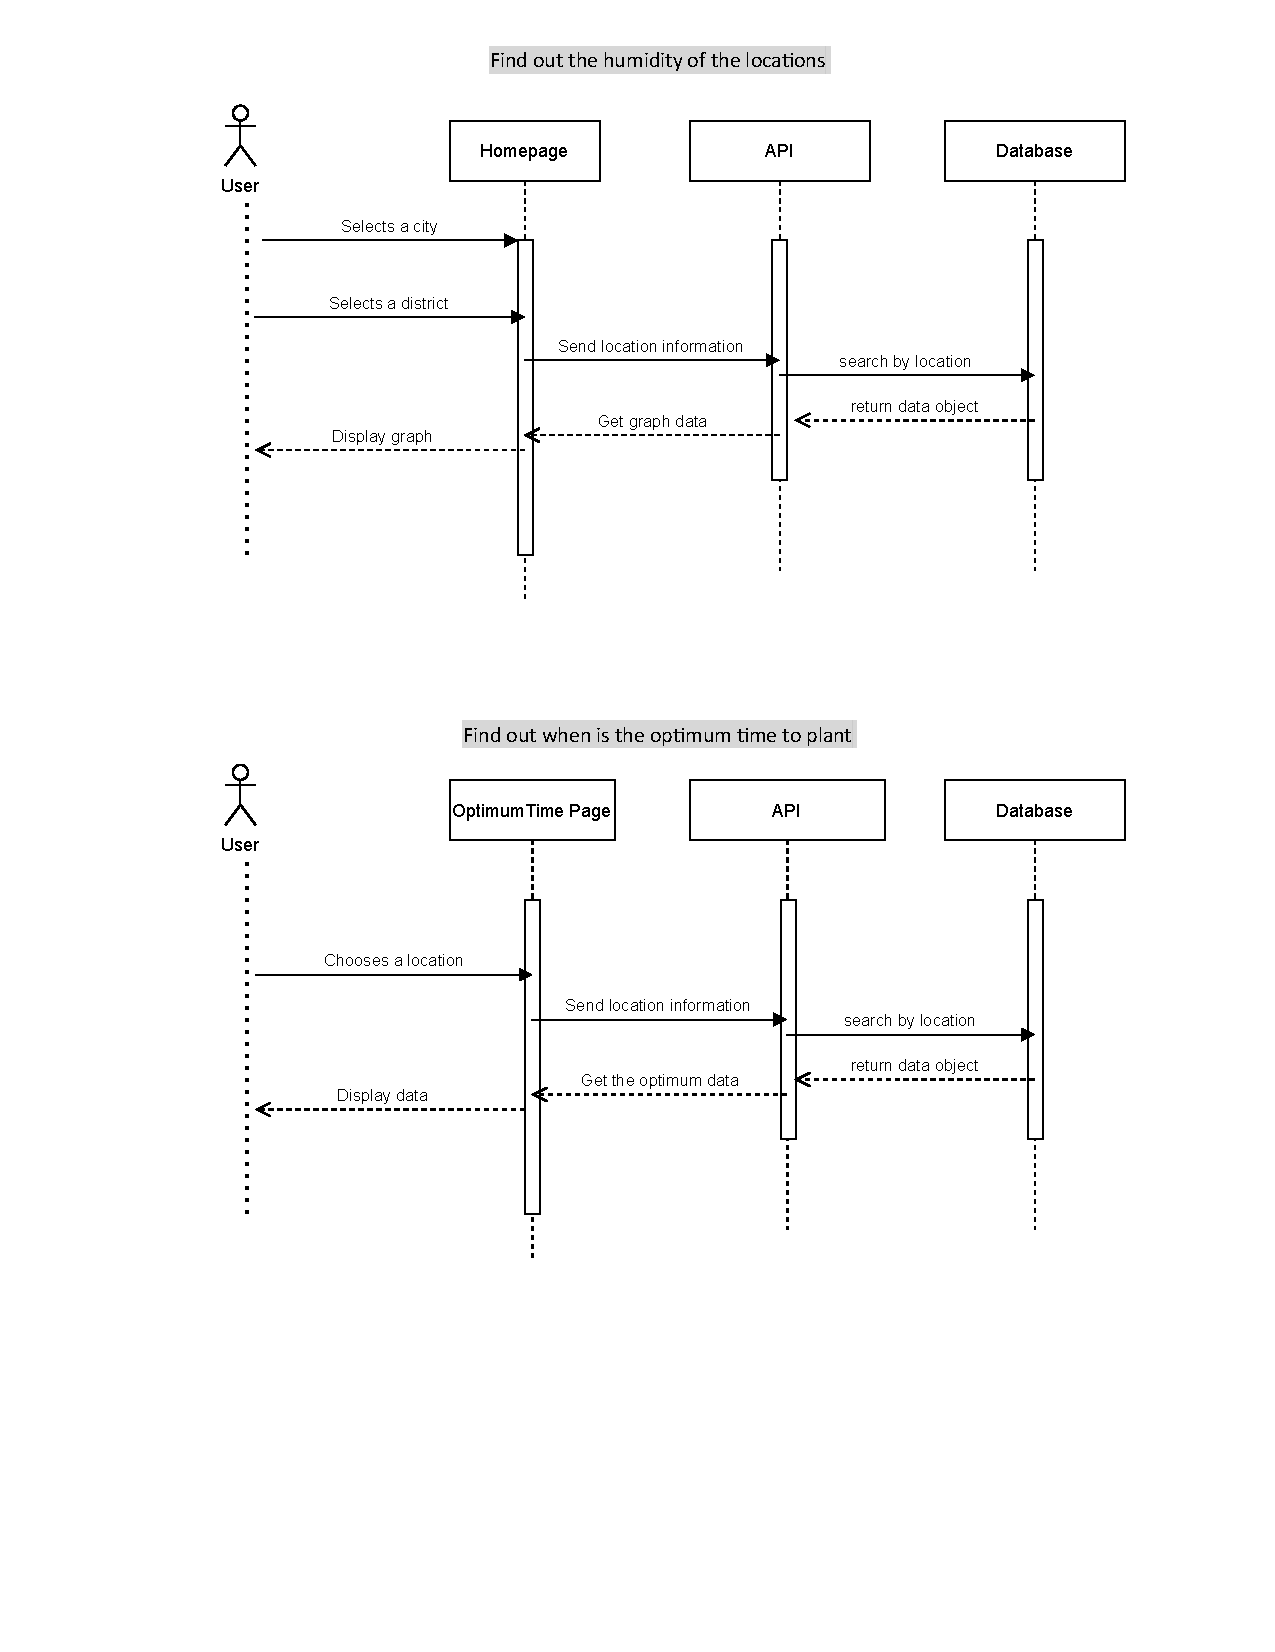
\includepdf[pages=-]{Sequence_Diagram.drawio_1.pdf}


    \title{\textbf{Flow Chart}}

\begin{figure}[H]
	\centering
	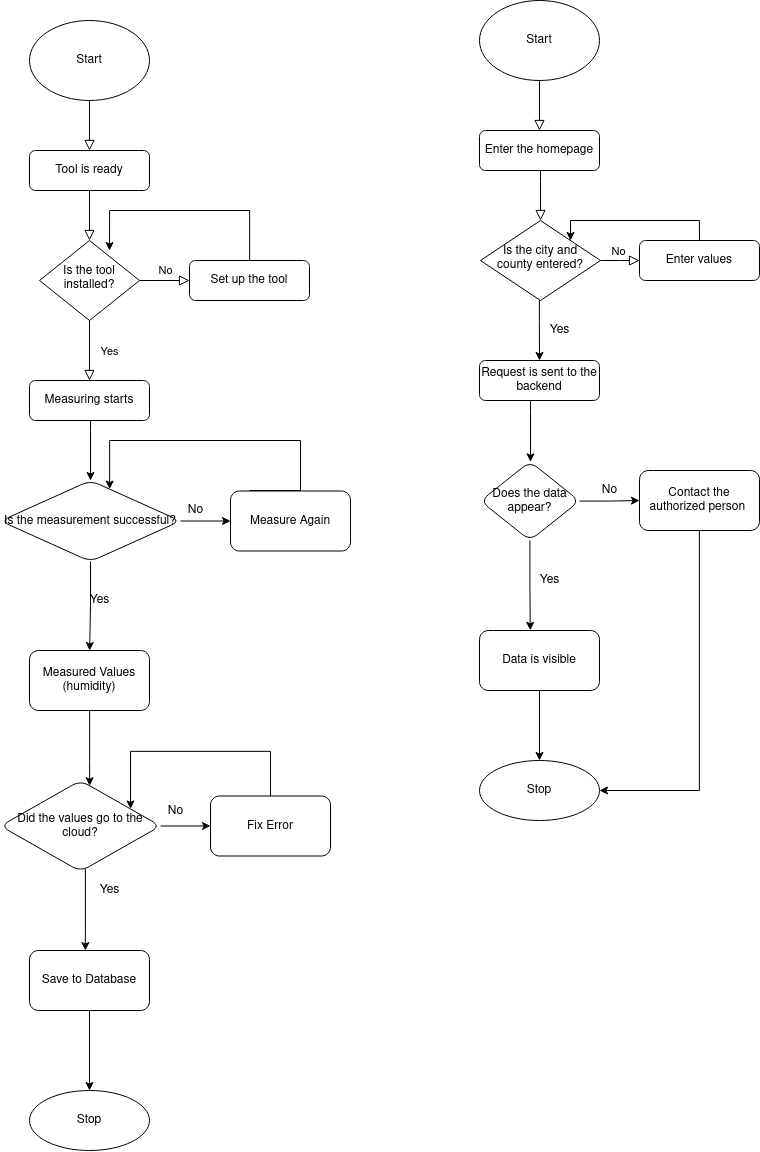
\includegraphics[ scale = 0.5]{flowchart.png}\newline\newline\newline
\end{figure}

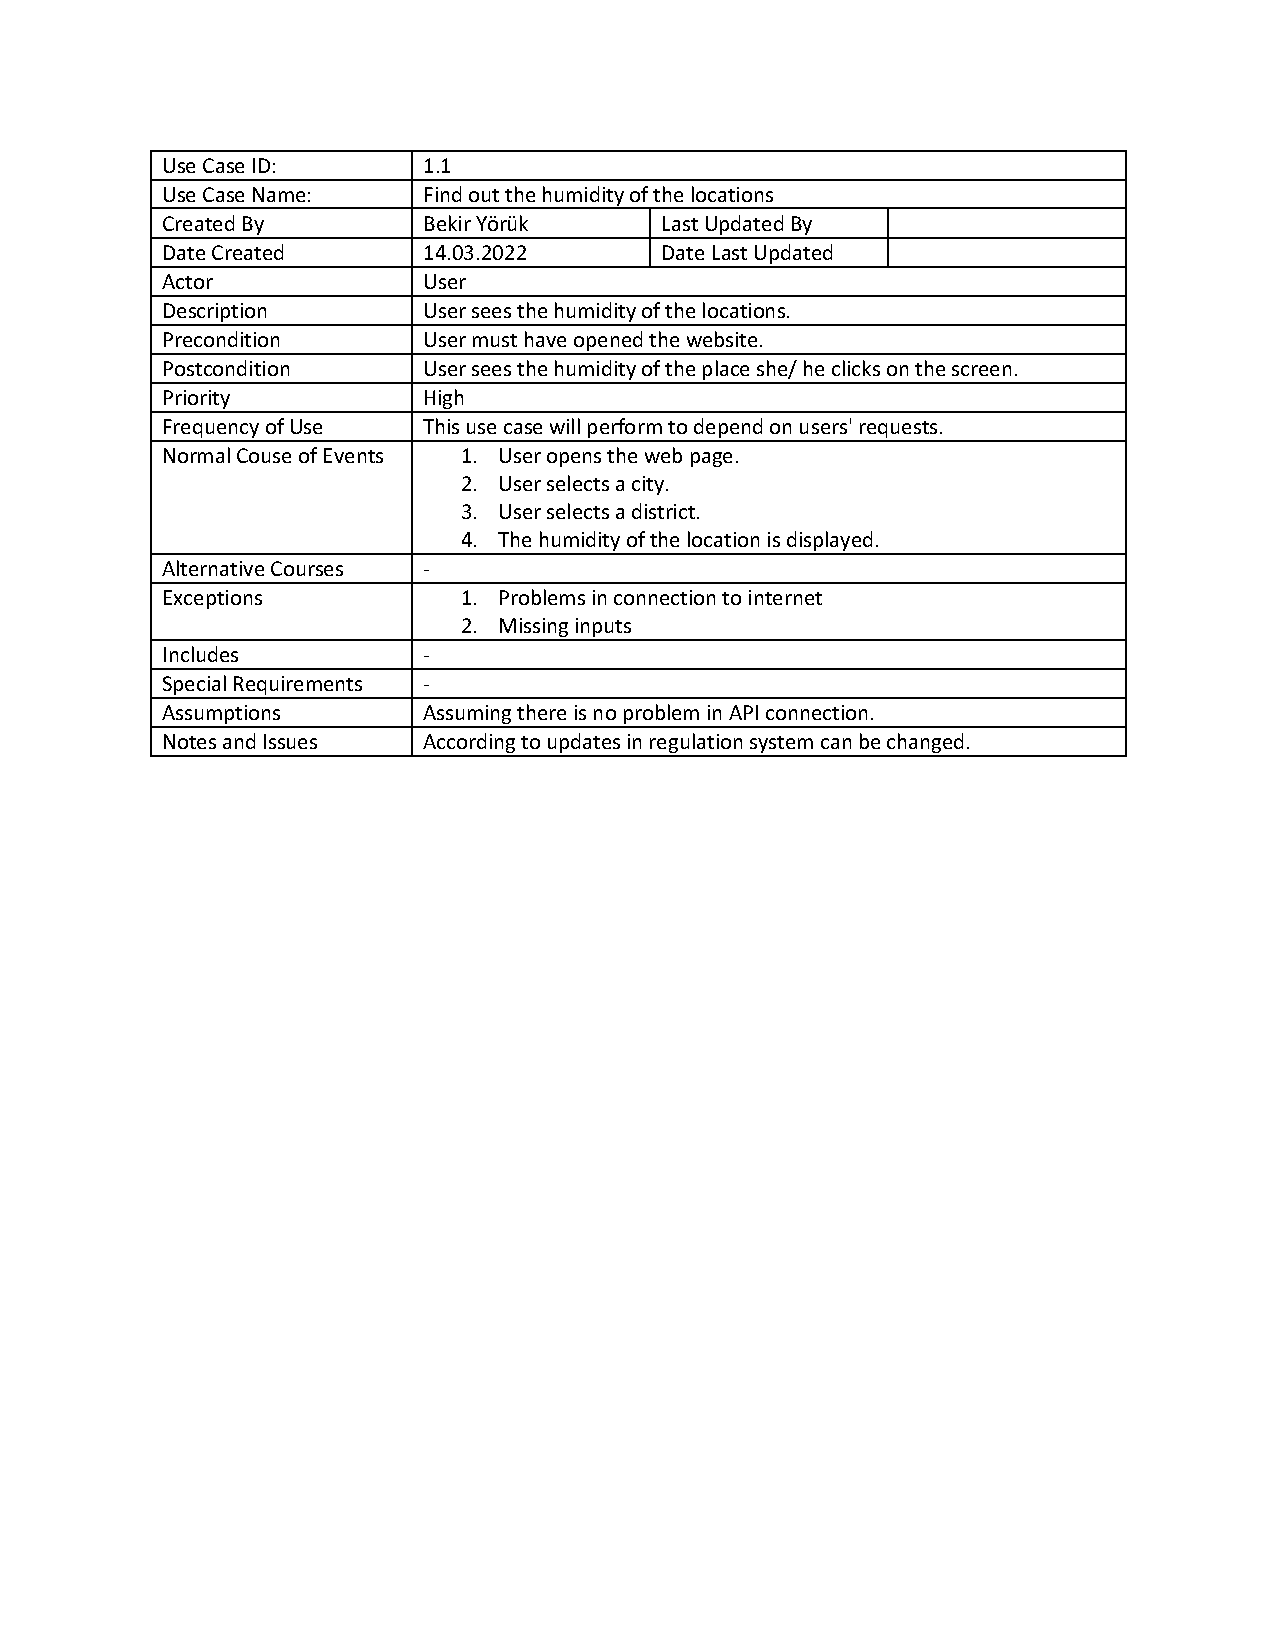
\includepdf[pages=-]{Use_Cases.pdf}

\begin{figure}[H]
	\centering
	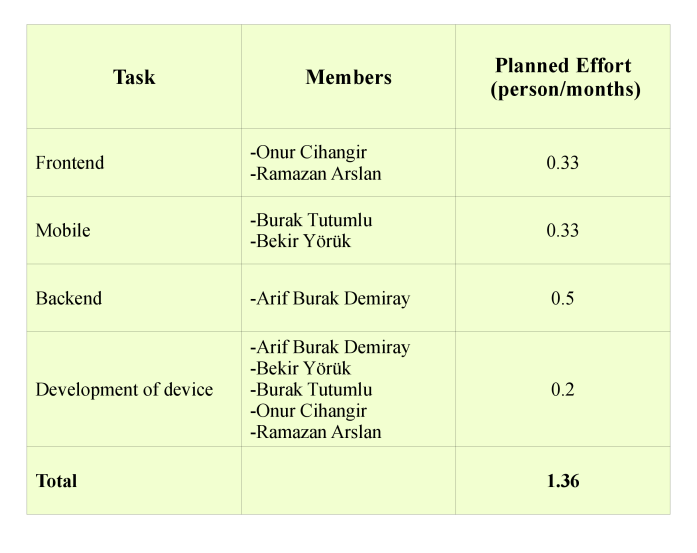
\includegraphics[ scale = 0.5]{responsibility_and_efforts.png}\newline\newline\newline
\end{figure}

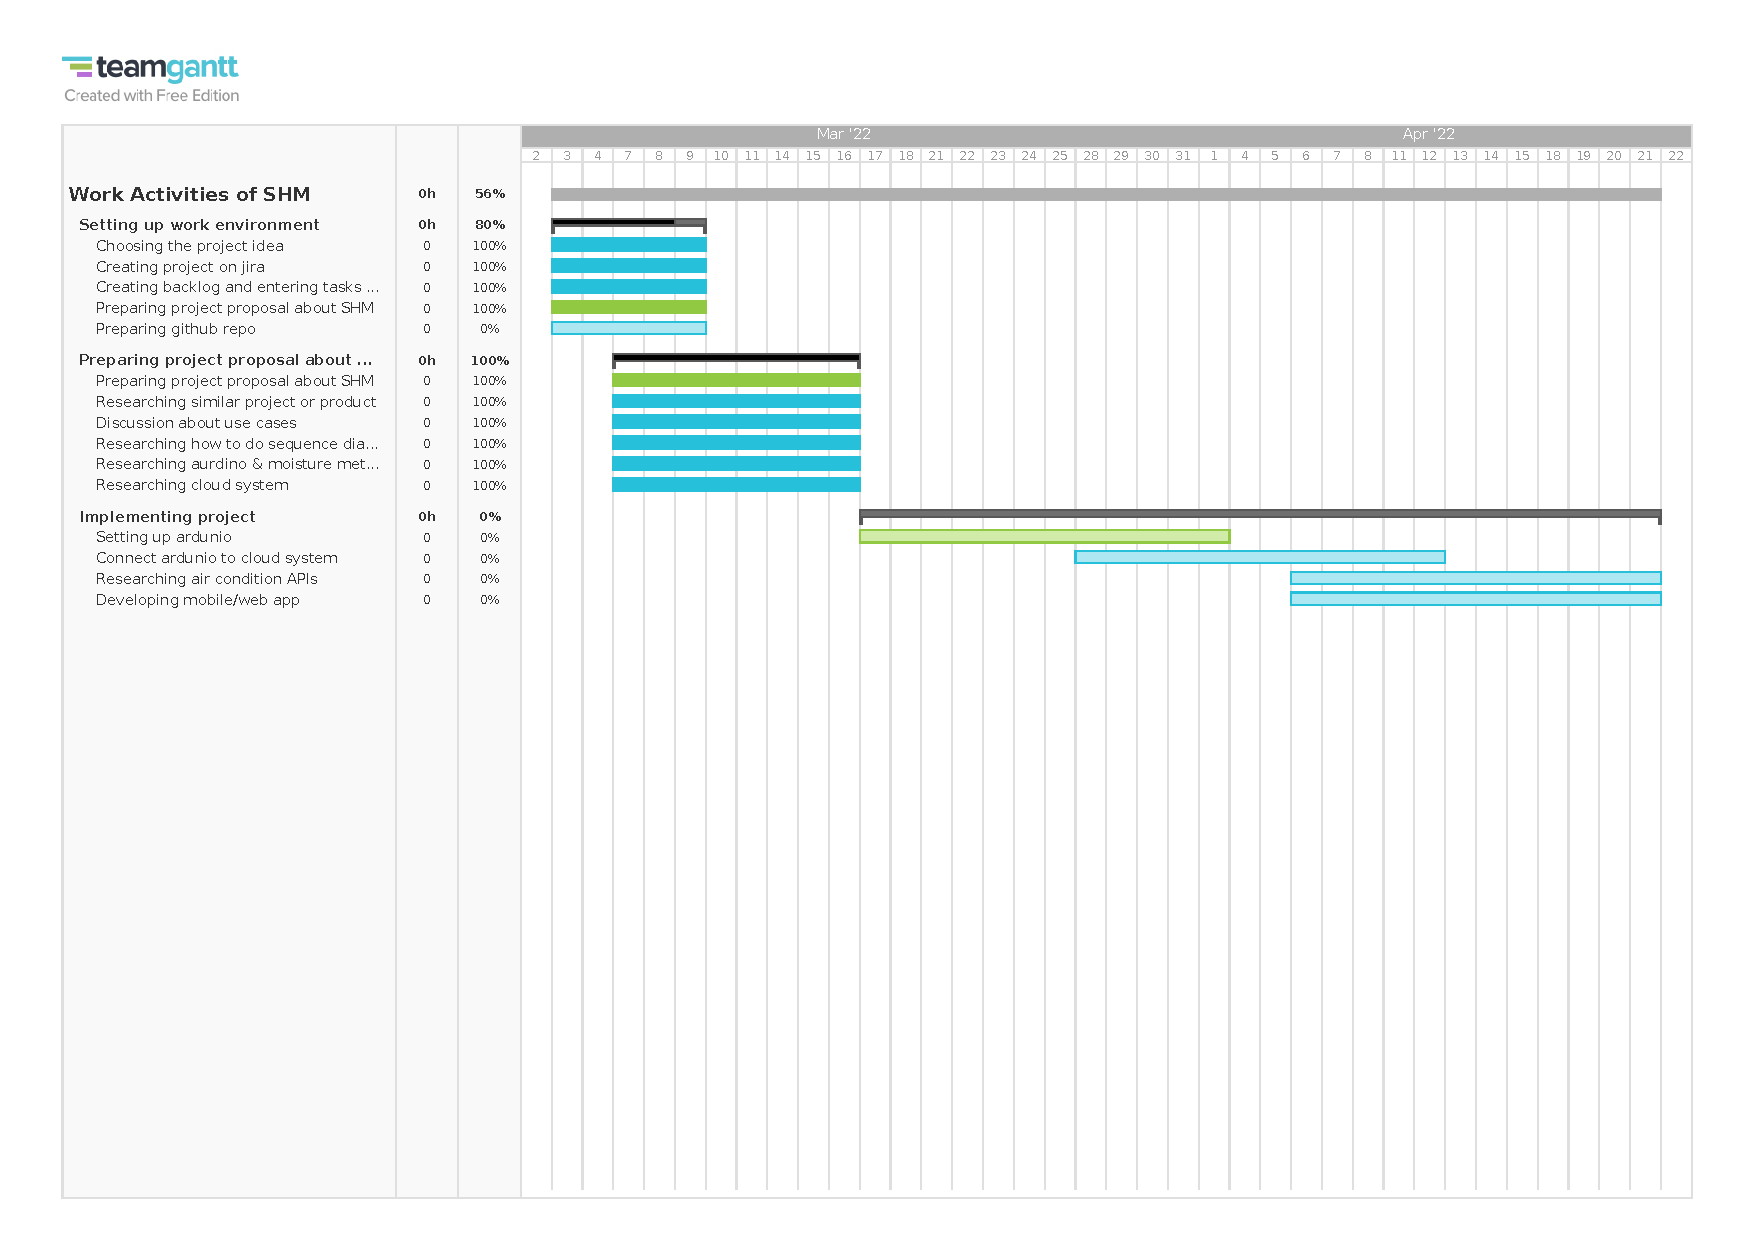
\includepdf[pages=-]{Work_Activities_of_SHM.pdf}

\section{Tools, Software, Hardware}
We are going to use Jira for project management and GitHub for version control and code control. We are going to use React for the website. Backend is going to be spring boot. Mobile is going to be React Native. Database is going to be MySQL because it is on free tier in AWS. Also, we are going to use AWS for the backend deployment and Vercel for the web deployment. We are going to use Ardunio for the soil humidity meter. It consist of lcd, buzzer, led lights, esp8266, ardunio uno, dht11 humidity sensor. According to [1], dht11 is capable of handling humidity between 0 and 50 celsius. And, humidity probes' radius is approximately 2 meter. Other option is FC-28 Hygrometer sensor and it will be the our selection when measuring the humidity. Because it is a hand tool, users can easily measure humidity across fields. We plan to connect public wireless connections for now.

\begin{figure}[H]
	\centering
	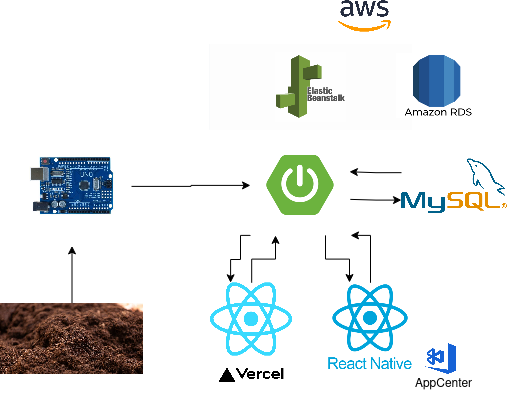
\includegraphics[ scale = 0.6]{sistemspecv3} 
\end{figure}

Below diagram will be the hand-tool circuit diagram:

\begin{figure}[H]
	\centering
	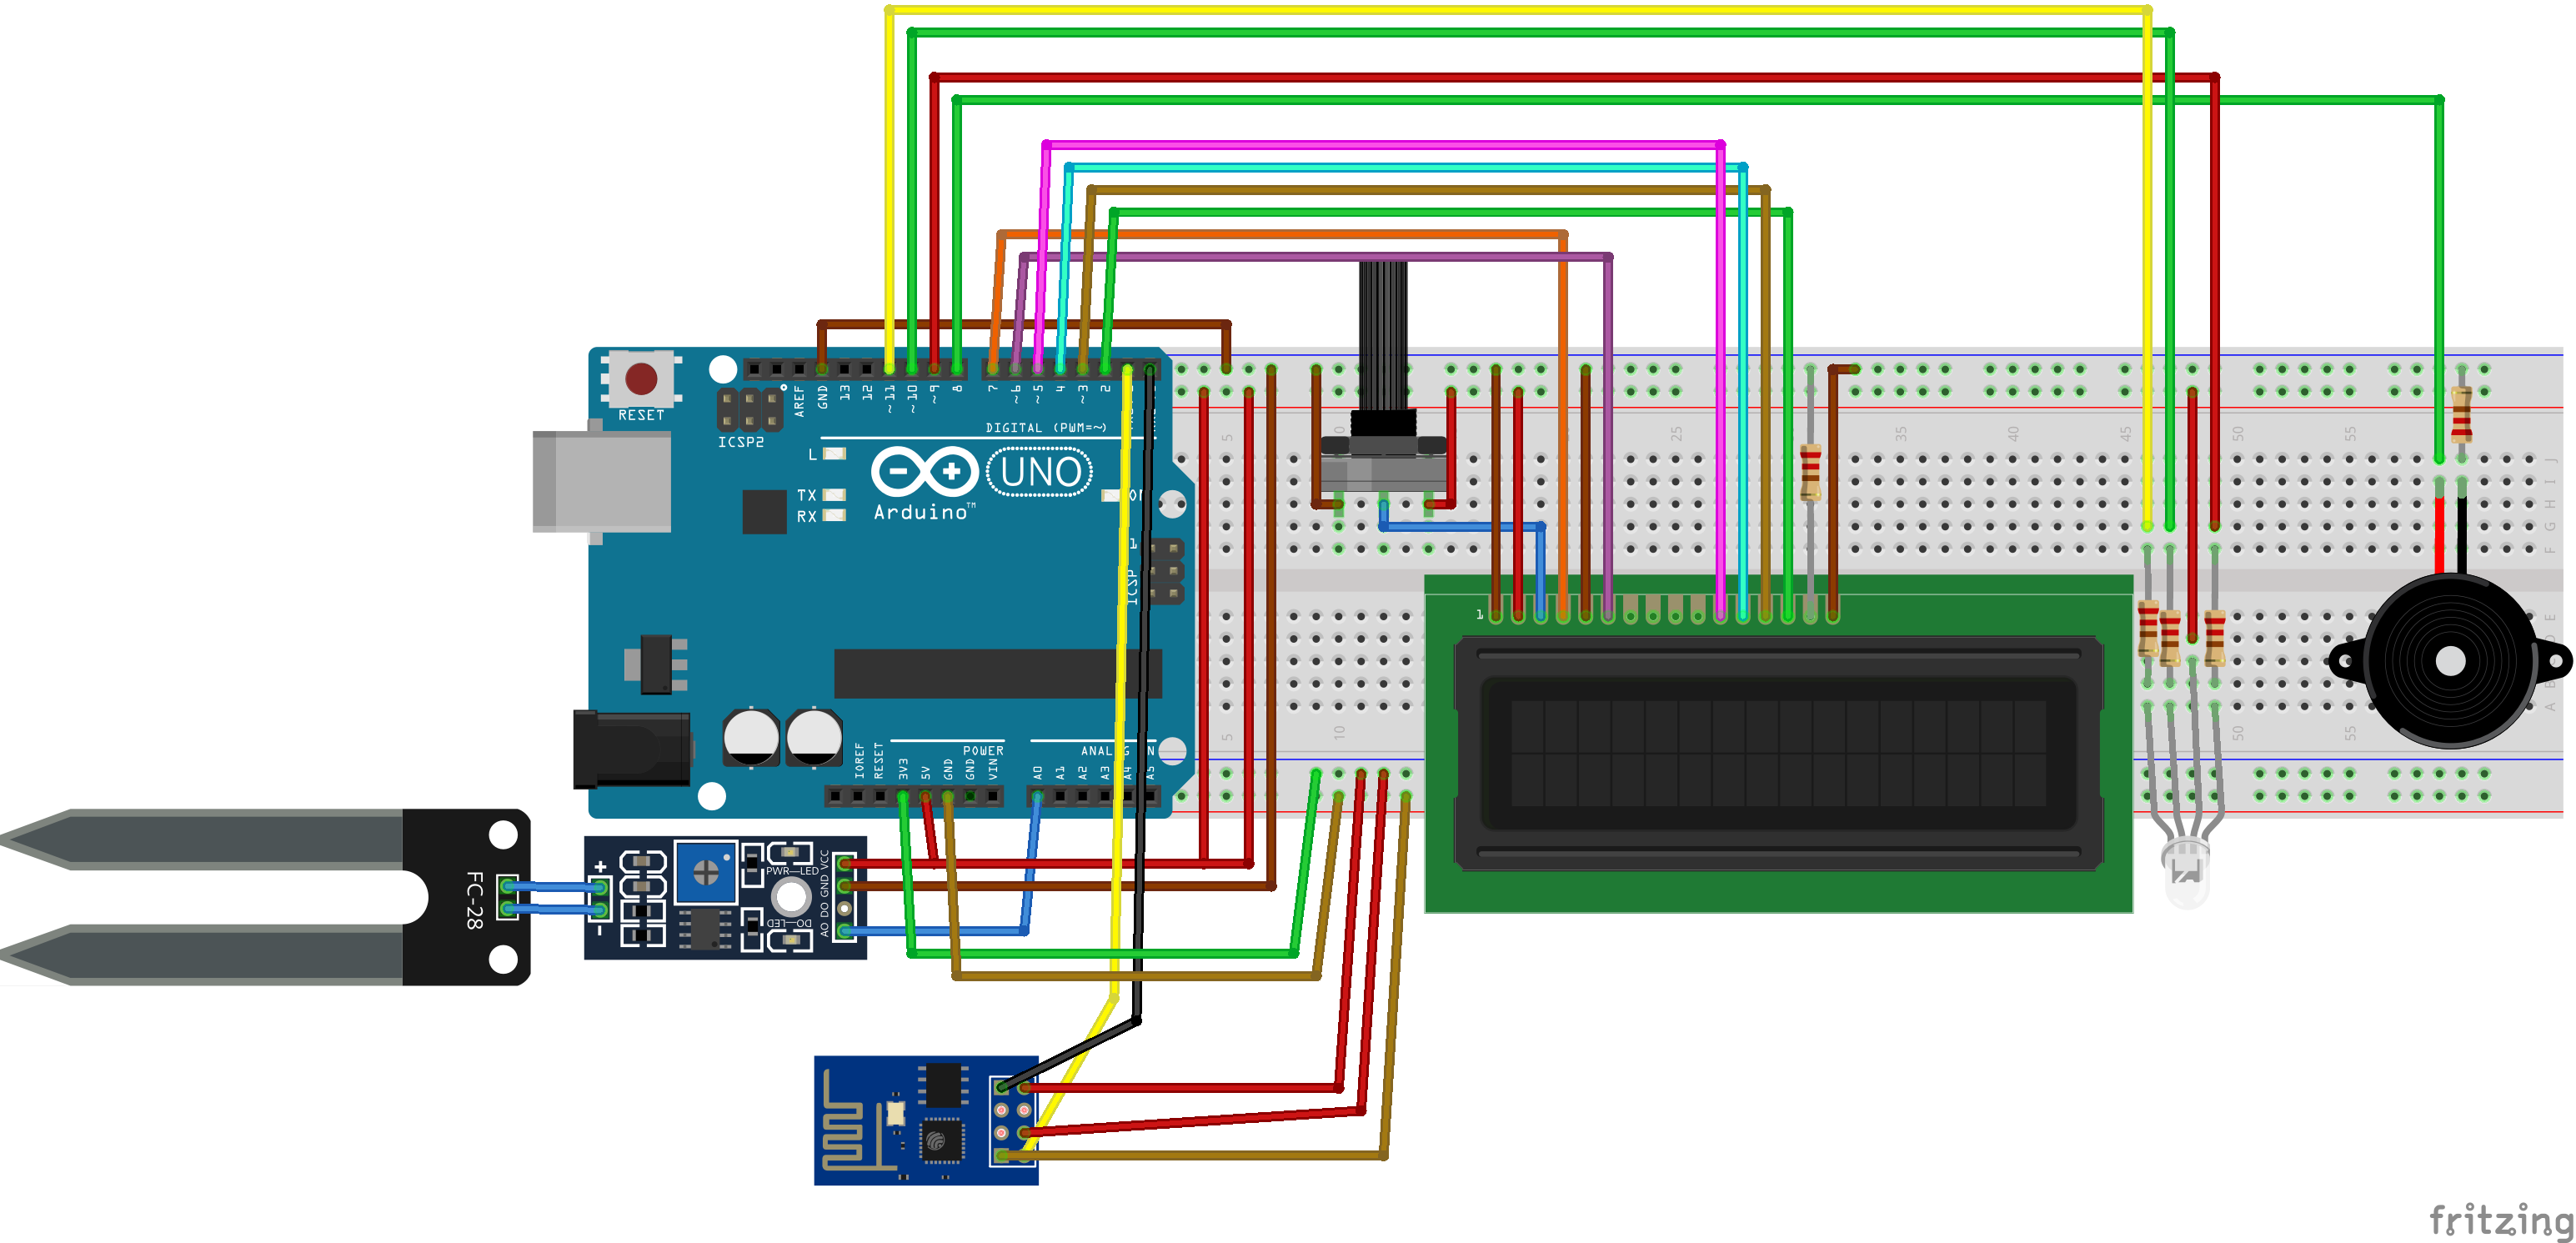
\includegraphics[ scale = 0.6]{Devre_bb.png} 
\end{figure}

\begin{figure}[H]
	\centering
	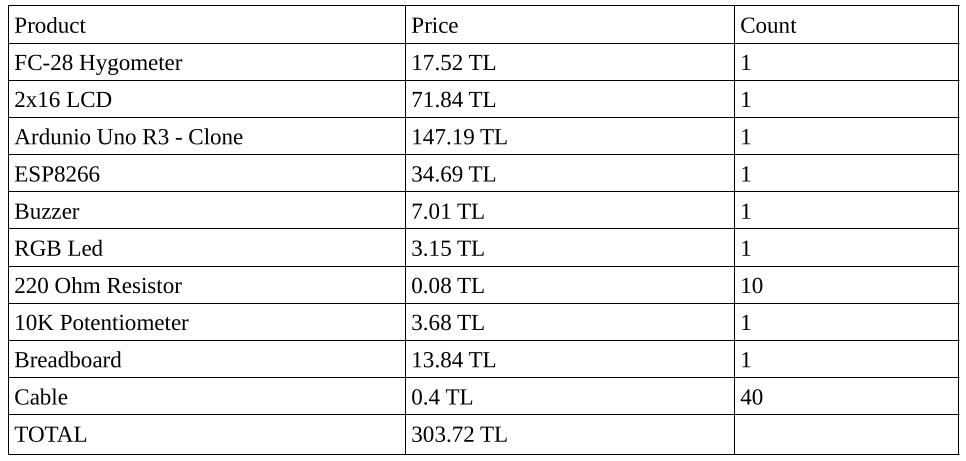
\includegraphics[ scale = 0.5]{image.png} 
\end{figure}


\section{Experiments\&Results, Test Phases}
Our garden is going to be the testing ground for this. We are going to use the device in three soil conditions: dry, wet and saturated with water. We plan to measure the humidity percentage and observe that the results go to our cloud server and access the results from the website. These test cases can be repeated morning, noon and evening. Response and request duration must be one second at maximum threshold. 
\section{Weekly Schedule}

\href{https://discord.gg/yA3v3fwm}{Discord} 
    
\href{https://eye-tracking-iyte.atlassian.net/jira/software/projects/SHM/boards/2}{Jira} 
    
\href{https://github.com/orgs/SoilHumidityMeter/dashboard}{GitHub} 


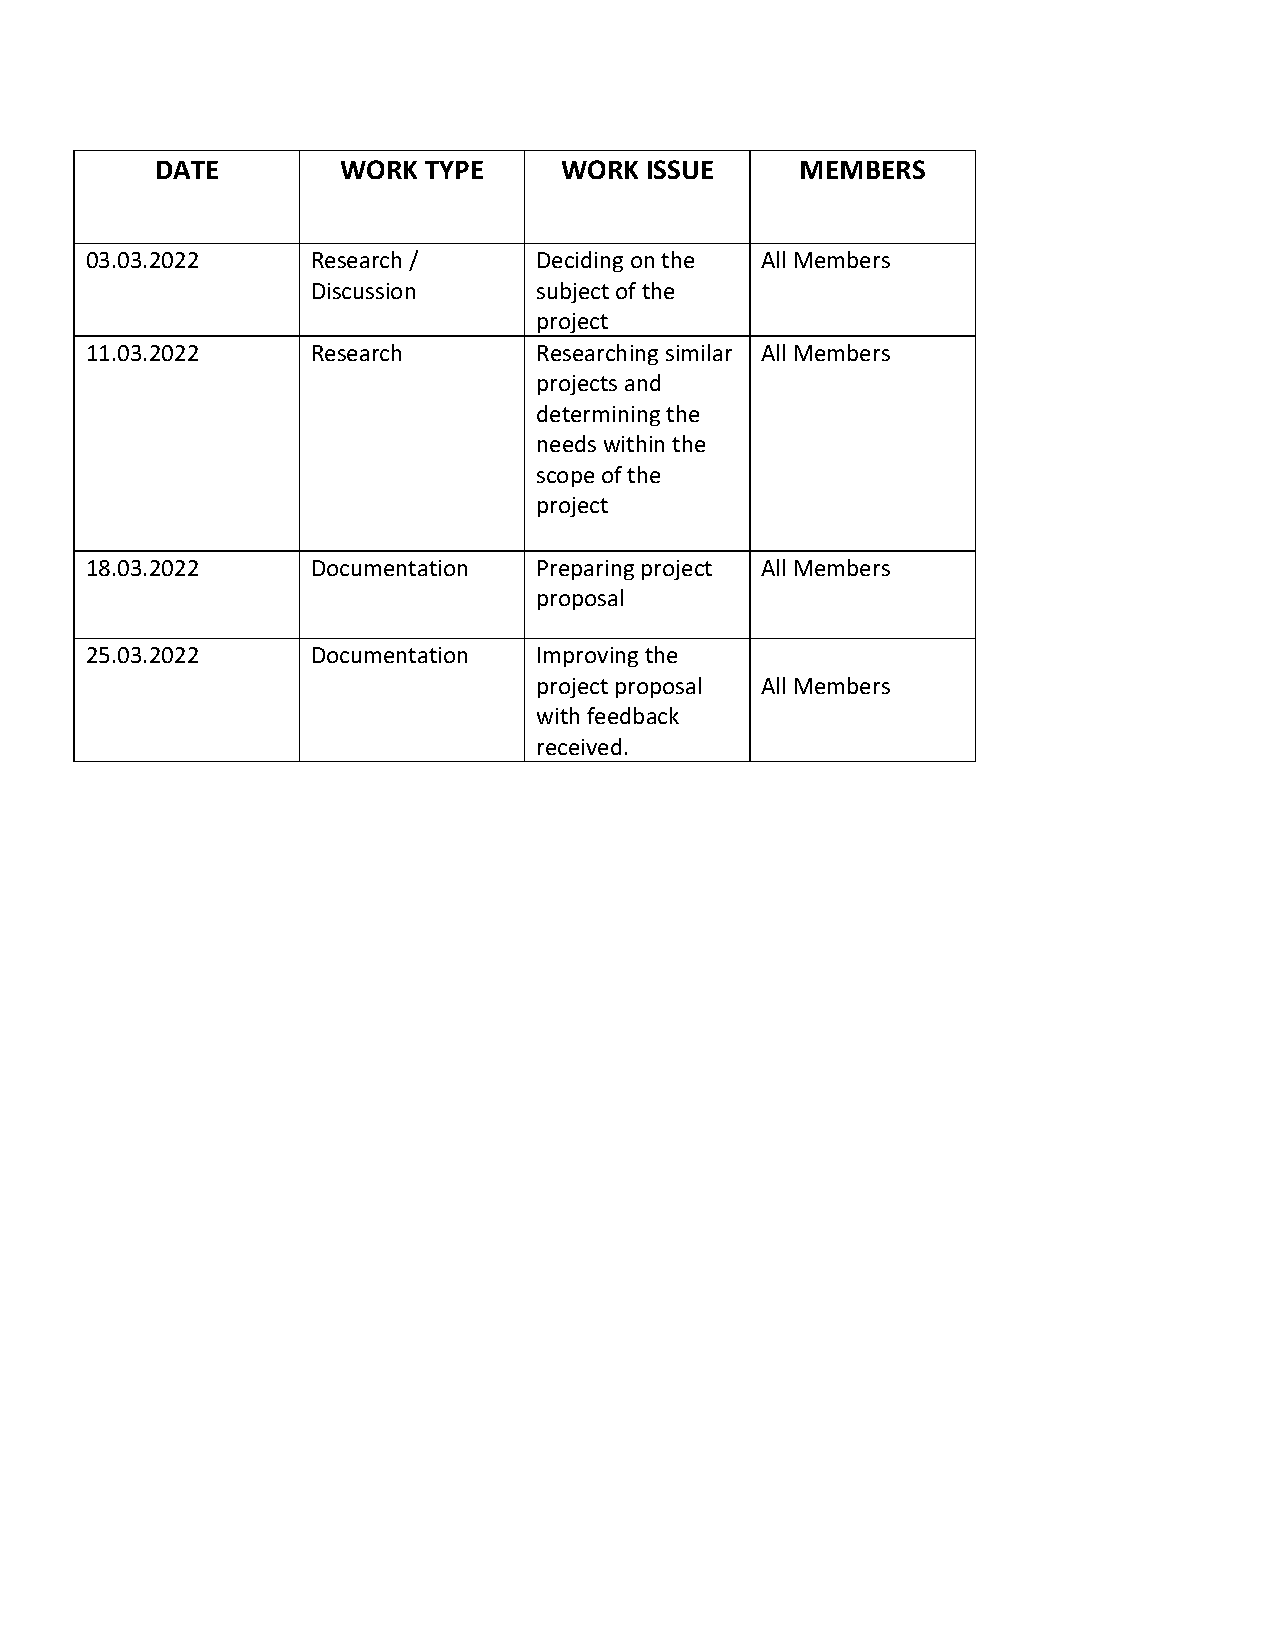
\includepdf[pages=-]{weekly_schedule.pdf}


\section{References}

[1]
W. Gay, “DHT11 sensor,” in Advanced Raspberry Pi, Springer, 2018, pp. 399–418.

[2]
J. L. Harper and R. Benton, “The behaviour of seeds in soil: II. The germination of seeds on the surface of a water supplying substrate,” The Journal of Ecology, pp. 151–166, 1966.


[3]
A. Uytun, B. Pekey, and M. Kalemci, “Toprak nemi ölçümleri,” Ulusal Ölçübilim Kongresi, pp. 26–28, 2013.


[4]
Y. A. K. Utama, Y. Widianto, Y. Hari, and M. Habiburrahman, “Design of weather monitoring sensors and soil humidity in agriculture using internet of things (IOT),” Transactions on Machine Learning and Artificial Intelligence, vol. 7, no. 1, pp. 10–20, 2019.



\end{document}


